\documentclass[border=0pt]{standalone}

\usepackage[sc]{mathpazo}
\linespread{1.05}
\usepackage[table]{xcolor}
\definecolor{petrol}{RGB}{127,173,198}

\usepackage{tikz}
\usetikzlibrary{
  calc,
  positioning,
  shapes.callouts,
  decorations.pathreplacing,
  decorations.pathmorphing,
  arrows.meta
}


\def\niterate{60}
\tikzset{
  put dots/.style={
    /utils/exec={
      \pgfmathsetmacro\a{1.8 + rnd*2}   
      \pgfmathsetmacro\b{1 + rnd*5}     
      \pgfmathsetmacro\c{1 + rnd*1}     
      \pgfmathsetmacro\d{rnd*1.5}       
      \pgfmathsetmacro\dark{70 + rnd*30}
    },
    line width=\a pt,
    dash pattern=on \b pt off \c pt,
    dash phase=\c pt * rnd,
    shift={(rnd*360:\d pt)},
    line cap=round,
    red!\dark!black,
    opacity=0.9
  },
  chalkstroke/.style={
    decorate,
    decoration={
      show path construction,
      lineto code={
        \foreach \i in {1,...,\niterate} {
          \draw[put dots]
            (\tikzinputsegmentfirst) -- (\tikzinputsegmentlast);
        }
      },
      curveto code={
        \foreach \i in {1,...,\niterate} {
          \draw[put dots]
            (\tikzinputsegmentfirst)
            .. controls (\tikzinputsegmentsupporta)
                       and (\tikzinputsegmentsupportb)
            .. (\tikzinputsegmentlast);
        }
      }
    }
  }
}

\begin{document}
\small
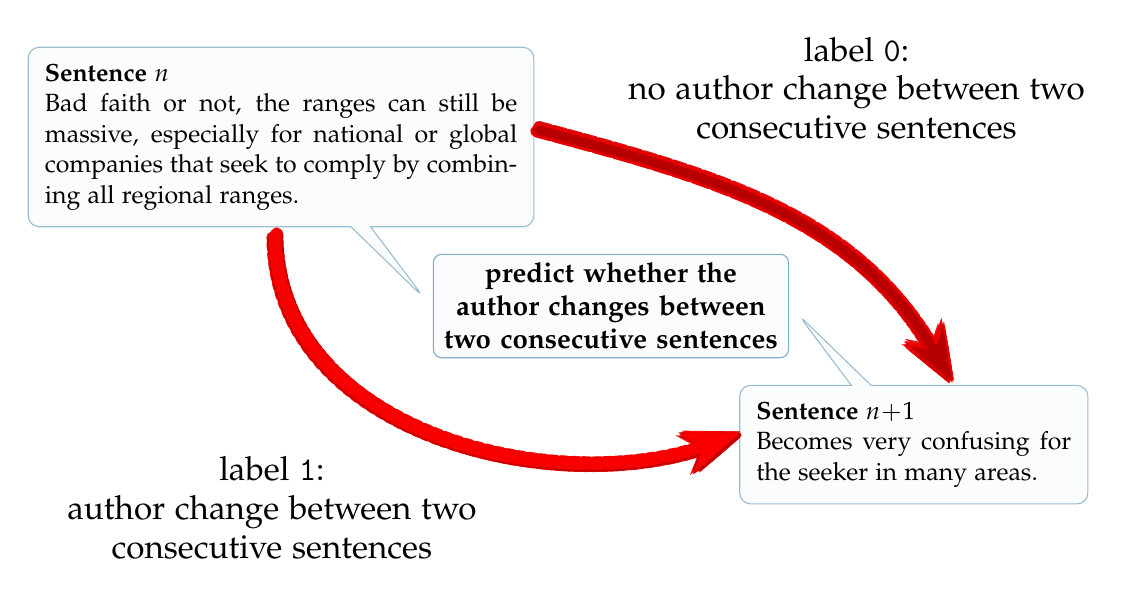
\begin{tikzpicture}[
  bubble/.style={
    rectangle callout,
    draw=petrol!80,
    fill=petrol!3,
    rounded corners=4pt,
    text width=6cm,
    inner sep=6pt,
    align=justify,
    font=\small
  },
   bubble2/.style={
    rectangle callout,
    draw=petrol!80,
    fill=petrol!3,
    rounded corners=4pt,
    text width=4cm,
    inner sep=6pt,
    align=justify,
    font=\small
  }
]


  \node[bubble,callout relative pointer={(0.8,-0.9)},anchor=north west]
    (msg1) at (0,0)
  {
    \textbf{Sentence $n$}\\Bad faith or not, the ranges can still be massive, especially for national or global companies that seek to comply by combining all regional ranges.
  };


  \node[bubble2,callout relative pointer={(-0.8,0.9)},
        below right=2cm and 2.6cm of msg1.south east]
    (msg2)
  {
    \textbf{Sentence $n\!+\!1$}\\Becomes very confusing for the seeker in many areas.
  };

  
  \coordinate (A1) at ($(msg1.pointer)+(-1.95,0.85)$);
  \coordinate (B1) at ($(msg2.pointer)+(-0.7,-1.6)$);

  \coordinate (A2) at ($(msg1.pointer)+(1.4,2.2)$);
  \coordinate (B2) at ($(msg2.pointer)+(2,-0.9)$);


  \draw[chalkstroke,->,>=Stealth] (A1) to[out=-90,in=200] (B1);
  \draw[chalkstroke,->,>=Stealth] (A2) to[out=-15,in=120] (B2);


  \path (A1) to[out=-90,in=200] coordinate[midway] (M1) (B1);
  \node[sloped,above,align=center,font=\large,xshift=-2.1cm,yshift=-1.7cm] at (M1) {label \texttt{1}:\\ author change between two\\ consecutive sentences};

  \path (A2) to[out=-15,in=120] coordinate[midway] (M2) (B2);
  \node[sloped,above,align=center,font=\large, xshift=1cm,yshift=0.8cm] at (M2) {label \texttt{0}:\\ no author change between two\\ consecutive sentences};
  
  \coordinate (midAll) at ($(msg1.pointer)!0.5!(msg2.pointer)$);


\node[
  draw=petrol!99,
  fill=petrol!5,
  rounded corners=3pt,
  inner sep=3pt,
  font=\normalsize,
  align=center,
  text width=4.3cm
] at (midAll)
{%
  \textbf{predict whether the}\\
  \textbf{author changes between two consecutive sentences}%
};

\end{tikzpicture}
\end{document}